\chapter{Conic Programming}

\paragraph{Announcement}
In the remaining classes, we will focus on the last topic: \textit{conic programming}.

\section{Introduction to Formulations}

\paragraph{General Conic Programming Problem}
Given $\bm A_i\in\mathbb{R}^{m\times n},\bm b_i\in\mathbb{R}^m,\bm c\in\mathbb{R}^{n\times p}$, and a \emph{closed convex cone} $\mathcal{K}\subseteq\mathbb{R}^n$, the general conic programming problem aims to solve
\begin{equation}\label{Eq:13:1}
\begin{array}{ll}
\min_{\bm X\in\mathbb{R}^{n\times p}}&\inp{\bm C}{\bm X}\\
\mbox{such that}&\bm A_i\bm X=\bm b_i,\\
&\bm X\in\mathcal{K}
\end{array}
\end{equation}
\begin{definition}[Cone]
A subset $\mathcal{K}$ for a vector space $V$ is a (closed) \emph{cone} if for each $\bm x\in\mathcal{K}$, we have $\alpha\bm x\in\mathcal{K}$ for $\forall\alpha>0$.
\end{definition}

Let's discuss some special cases for conic programming:
\begin{enumerate}
\item
Linear Programming: For $\bm A\in\mathbb{R}^{m\times n},\bm b\in\mathbb{R}^m,\bm c\in\mathbb{R}^n$, consider
\begin{equation}\label{Eq:13:2}
\begin{array}{ll}
\min&\inp{\bm c}{\bm x}\\
\mbox{such that}&\bm A\bm x=\bm b\\
&\bm x\ge0
\end{array}
\end{equation}
Here the LP problem is by setting $p=1$ and $\mathcal{K}=\{\bm x\mid\bm x\ge0\}$ in (\ref{Eq:13:1}). We can also construct the dual for LP problem:
\begin{equation}\label{Eq:13:3}
\left\{
\begin{array}{ll}
\min&\inp{\bm b}{\bm y}\\
\mbox{such that}&\bm A\trans\bm y\le\bm c
\end{array}
\right.
\Longleftrightarrow
\left\{
\begin{array}{ll}
\min&\inp{\bm b}{\bm y}\\
\mbox{such that}&\bm A\trans\bm y+\bm s=\bm c\\
&\bm s\ge0
\end{array}
\right.
\end{equation}
\item
Semidefinite Programming (SDP): Given $\bm A_i\in\mathbb{S}^p$ for $i=1,\dots,m$, $\bm b_i\in\mathbb{R}^m,\bm C\in\mathbb{S}^p$, consider the problem
\begin{equation}\label{Eq:13:4}
\begin{array}{ll}
\min_{\bm X}&\inp{\bm C}{\bm X}\\
&\inp{\bm A_i}{\bm X}=\bm b_i,\quad i=1,\dots,m\\
&\bm X\succeq0
\end{array}
\end{equation}
Here the SDP problem is by setting $m=n=p$, and $\mathcal{K}=\{\bm X\mid\bm X\succeq0\}.$ We can construct the SDP in dual form:
\begin{equation}\label{Eq:13:5}
\left\{
\begin{array}{ll}
\max_{\bm y}&\inp{\bm b}{\bm y}\\
&\sum_{i}y_i\bm A_i\succeq\bm C
\end{array}
\right.
\Longleftrightarrow
\left\{
\begin{array}{ll}
\max_{\bm y,\bm S}&\inp{\bm b}{\bm y}\\
&\sum_{i}y_i\bm A_i+\bm S=\bm C\\
&\bm S\succeq0
\end{array}
\right.
\end{equation}
\item
Second Order Conic Programming (SOCP): Given $\bm A_j\in\mathbb{R}^{m\times(1+n_j)},\bm c_j\in\mathbb{R}^{1+n_j},j=1,\dots,k$, and $\bm b\in\mathbb{R}^m$, consider
\begin{equation}\label{Eq:13:6}
\begin{array}{ll}
\min_{x_1,\dots,x_k}&\bm c_1\trans x_1+\cdots+\bm c_k\trans x_k\\
&\bm A_1x_1+\cdots+\bm A_kx_k=\bm b\\
&x_j\in\mathcal{S}_2^{1+n_j},\quad j=1,\dots,k
\end{array}
\end{equation}
where $\mathcal{S}_2^{1+q}$ is the \emph{second-order cone}:
\begin{figure}[H]
\centering
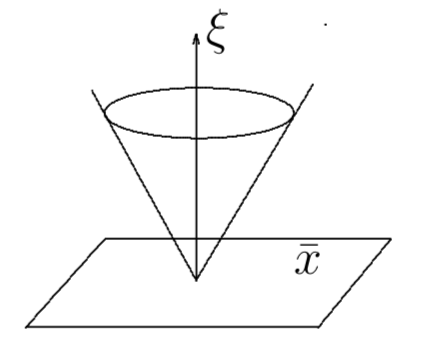
\includegraphics[width=10cm]{week13/SOCP}
\caption{Illustration for second-order cone $\mathcal{S}_2^{1+q}=\{\bm x:=(\xi;\bar{\bm x})\in\mathbb{R}^{1+q}\mid \xi\ge\|\bar{\bm x}\|_2\}$}
\end{figure}
You may also try to write this problem into standard conic programming form. The dual form is given by:
\begin{equation}\label{Eq:13:7}
\begin{array}{ll}
\max_{\bm y}&\inp{\bm b}{\bm y}\\
&c_j-\bm A_j\trans\bm y\in\mathcal{S}_2^{1+n_j},\quad j=1,\dots,k
\end{array}
\end{equation}
Or equivalently,
\begin{equation}\label{Eq:13:8}
\begin{array}{ll}
\max_{\bm y,\bm s_1,\dots,\bm s_k}&\inp{\bm b}{\bm y}\\
&c_j-\bm A_j\trans\bm y+\bm s_i=\bm c_i,\quad j=1,\dots,k\\
&s_j\in\mathcal{S}_2^{1+n_j},\quad j=1,\dots,k
\end{array}
\end{equation}








\end{enumerate}

\paragraph{Conic problem in dual form} How do we construct the (\ref{Eq:13:1}) in dual form? We need the dual cone:
\[
\mathcal{K}^*=\{\bm s\in\mathbb{R}^n\mid\inp{\bm s}{\bm x}\ge0,\forall\bm x\in\mathcal{K}\}
\]
Thus we define the dual conic programming:
\begin{equation}\label{Eq:13:9}
\begin{array}{ll}
\max_{\bm y,\bm s}&\sum_i\inp{\bm b_i}{\bm y_i}\\
&\bm A_i^*\bm y_i+\bm s_i=\bm c\\
&\bm s_i\in\mathcal{K}^*
\end{array}
\end{equation}



\section{Weak Duality}
\paragraph{Weak Duality for LP}
If $\bm x$ is feasible for (\ref{Eq:13:2}) and $(\bm y,\bm s)$ is feasible for (\ref{Eq:13:3}), then
\begin{align*}
\bm c\trans\bm x-\bm b\trans\bm y&=(\bm A\trans\bm y+\bm s)\trans\bm x-(\bm A\bm x)\trans\bm y\\
&=\bm s\trans\bm x\ge0
\end{align*}
\paragraph{Weak Duality for SDP}
For $\bm X$ feasible in (\ref{Eq:13:4}) and $(\bm y,\bm S)$ feasible for (\ref{Eq:13:5}), we have
\begin{align*}
\inp{\bm C}{\bm X}-\bm b\trans\bm y&=\inp{\sum y_i\bm A_i+\bm S}{\bm X}-(\inp{\bm A_i}{\bm X}_{i=1}^m)\trans\bm y\\
&=\inp{(\sum y_i\bm A_i)}{\bm X}+\inp{\bm S}{\bm X}-\sum y_i(\inp{\bm A_i}{\bm X})\\
&=\inp{\bm S}{\bm X}\ge0
\end{align*}
\paragraph{Weak Duality for SOCP}
For $( x_1,\dots, x_k)$ feasible for (\ref{Eq:13:6}) and $(\bm y,(s_1,\dots,s_k))$ feasible for (\ref{Eq:13:7}), we have
\begin{align*}
\sum\bm c_j\trans x_j-\bm b\trans\bm y&=\sum(\bm A_j\trans\bm y+s_j)\trans x_j-(\sum\bm A_j x_j)\trans\bm y\\
&=\sum s_j\trans x_j\ge0
\end{align*}
\begin{remark}
\begin{enumerate}
\item
The spd cone in (\ref{Eq:13:4}) is self-dual, i.e., $\mathcal{K}=\mathcal{K}^*$. 
\item
The weak duality holds for all cases, which suggests that it is worthwhile to consider primal and dual problem together. In many cases, strong duality holds (not all cases). Once the strong duality holds, we could solve the primal and dual problem by interior point methods (remember assignment 5)?
\item
We will continue this topic in the next semester, i.e., CIE6110.
\end{enumerate}
\end{remark}























